%% AHAAR -- Kitchen System : IEEE-style Project Report
%% Compile with pdflatex, then bibtex, then pdflatex x2
%% Overleaf: upload main.tex, references.bib ; set compiler to pdfLaTeX
\documentclass[journal,onecolumn,12pt]{IEEEtran}

\usepackage[utf8]{inputenc}
\usepackage[T1]{fontenc}
\usepackage{graphicx}
\usepackage{amsmath,amssymb}
\usepackage{booktabs}
\usepackage{array}
\usepackage{url}
\usepackage{hyperref}
\usepackage{cite}
\usepackage{xcolor}
\usepackage{listings}
\usepackage{tabularx}

\hypersetup{colorlinks=true,linkcolor=blue,citecolor=blue,urlcolor=blue}

\lstset{
  basicstyle=\ttfamily\footnotesize,
  breaklines=true,
  columns=fullflexible,
  frame=single,
  showstringspaces=false
}

\begin{document}

\title{AHAAR: An AI-Driven Household Kitchen Assistant for Indian Cuisine with CGM-Aware Nutritional Personalization}

\author{%
  Rajiv Agarwal, Alan Joseph, Aryan Raina\\
  \textit{Group 19, Academic Year 2026--27}\\
  \textit{Project Guide: Ms.\ Sharlene Rebeiro}%
  \thanks{Source code: \url{https://github.com/workspace220106/Aahar-Kitchen-System}.
  Deployed demo: see the project page. All modules reported here are
  implemented, under test, and live on \texttt{main}.}
}

\markboth{AHAAR Project Report, 2026--27}{Agarwal \MakeLowercase{\textit{et al.}}: AHAAR -- Kitchen System}

\maketitle

%====================================================================
\begin{abstract}
Household food waste, repetitive cooking decisions, and the lack of
personalized dietary guidance remain persistent problems in Indian
kitchens. We present \textbf{AHAAR}, a progressive web application
that turns one photograph of the inside of a refrigerator into a
ranked set of culturally-appropriate recipes, portioned per family
member, re-ranked over time by each user's personal glycemic response
captured from a Continuous Glucose Monitor (CGM), and surfaced in ten
Indian languages. The system is end-to-end implemented: a YOLOv11m
detector fine-tuned on 107 Indian pantry classes runs behind a FastAPI
service and detects ingredients from a phone photograph; a 450-recipe
index pre-built from the IndianFoodDataset drives a client-side
scorer that combines pantry coverage with per-family-member
condition-aware penalties; dish-level nutrition from the Indian Food
Nutrition dataset (1{,}005 dishes) is attached to every recipe at
build time; a LibreView / Dexcom CSV ingest pipeline computes the
full ADA 2020 CGM metric suite in the browser; and a per-user
Glycemic Sensitivity Index learned from logged meals plus CGM windows
labels every future recipe with a predicted impact chip per
household member. We ground every design choice in ten peer-reviewed
IEEE papers spanning object detection, cross-modal recipe retrieval,
nutrition-aware recommendation, portion estimation, and
glucose-driven dietary monitoring, and describe the reproducible
training pipeline that evaluates four ablation cells
(YOLOv8m / YOLOv11m, with and without IndianFood20 two-stage
transfer) on an in-house fridge-interior dataset.
\end{abstract}

\begin{IEEEkeywords}
Food recognition, YOLO, Indian cuisine, recipe recommendation,
continuous glucose monitoring, personalized nutrition, deep learning,
progressive web application, internationalization.
\end{IEEEkeywords}

%====================================================================
\tableofcontents
\vspace{1em}
\hrule
\vspace{1em}

%====================================================================
\section{Introduction}
\IEEEPARstart{T}{he} question \textit{``what's for dinner?''} is asked
in roughly 300~million Indian households every day. The answer is
constrained by what is physically in the refrigerator, by regional
cuisine preferences, by the age and health status of each family
member, and -- for the roughly 101~million Indians living with
diabetes -- by the glycemic impact of the chosen meal. No existing
application addresses all four constraints simultaneously for Indian
cuisine.

AHAAR is organised as a sequence of pages that mirror the real
decision flow in a kitchen:
\textit{Fridge Scan $\rightarrow$ Detection $\rightarrow$ Pantry $\rightarrow$ Recipes $\rightarrow$ Family Portions $\rightarrow$ Weekly Plan $\rightarrow$ Cook-along $\rightarrow$ Health}.
Each page is backed by real data and real inference: the detector is
a trained YOLOv11m served from a FastAPI backend; the pantry page
drives an aggregated nutrition profile from the 1{,}005-dish Indian
Food Nutrition dataset; the health page ingests a Continuous Glucose
Monitor export (Abbott LibreView or Dexcom Clarity) and computes the
ADA~2020 CGM metric suite; and the recipe ranker learns a per-member
Glycemic Sensitivity Index from any logged meals aligned to CGM
windows, then uses it to flag high-impact dishes before they are cooked.

This report consolidates: (i) the ten IEEE references that anchor
each AHAAR subsystem; (ii) the implemented system architecture
(frontend, inference backend, data assets, training pipeline);
(iii) the proposed methodology for the primary ML contribution
(AHAAR-Fridge dataset + two-stage transfer YOLO training with a
four-cell ablation); (iv) the evaluation protocol that produces the
paper-cited metrics; and (v) a discussion of novelty, limitations,
and future work.

\textbf{Contributions.} We claim four contributions:
\begin{enumerate}
  \item A \emph{fridge-interior} Indian ingredient detection target
        and the training/evaluation pipeline to produce it -- distinct
        from existing \emph{plated-meal} Indian food datasets
        \cite{foodnet2017,indianfood10,indianfoodnet2023}.
  \item A light-and-sharpness pre-filter and a Lazy-Mode scan flow
        that turns image capture into ranked recipes in one tap, in
        the spirit of Inverse Cooking's set-prediction
        formulation~\cite{salvador2019inverse}.
  \item A dish-level nutrition enrichment pipeline that attaches
        per-serving nutrition from the Indian Food Nutrition dataset
        (1{,}005 dishes, 1{,}381 name variants) to every recipe at
        build time, driving the Pantry nutrition profile, Family
        portion totals, Recipes cards, Cook-along nutrition panel,
        and Health advice. 355 of 450 recipes (79\%) carry a
        matched nutrition row.
  \item A per-user Glycemic Sensitivity Index learned from logged
        meals and CGM windows that re-ranks future recipes for Indian
        cuisine, bridging the CGM-macronutrient literature
        \cite{huo2019cgm} with cross-modal recipe
        retrieval~\cite{marin2021recipe1m}.
\end{enumerate}

%====================================================================
\section{Related Work}
\label{sec:related}

We organise the related work along the five technical sub-problems
addressed by AHAAR.

\subsection{Object Detection and Food Recognition}

\textbf{YOLO}~\cite{redmon2016yolo} reframed object detection as a
single regression problem, predicting bounding boxes and class
probabilities in one network pass. This real-time, end-to-end approach
is directly suitable for on-device fridge scanning, where latency
budgets rule out two-stage detectors.

\textbf{FoodNet}~\cite{foodnet2017}, published in \textit{IEEE Signal
Processing Letters}, proposed an ensemble of deep CNNs for food
classification and -- importantly for us -- introduced the first
Indian food image database (50 classes, 100 images per class). It
established the baseline that domain-specific ensembles beat generic
backbones on Indian cuisine.

\textbf{IndianFood10 / YOLOv4 Platters}~\cite{indianfood10} applied
transfer learning with YOLOv4 to a 10-class dataset of staple Indian
plates and reported 91.8\% mAP, framing the central difficulties as
``lack of annotated Indian food datasets, non-distinct boundaries
between dishes on one plate, and high intra-class variation.''

\textbf{YOLO V11m Indian Cuisine}~\cite{yolov11indian2025}, the most
recent IEEE paper in this space, combined 17-class Indian food
detection with portion-based nutritional estimation and reached
\(\text{mAP}@50 = 0.94\). Its two-stage pipeline (detect $\rightarrow$
look up nutrition) is the architectural template we extend.

\subsection{Cross-Modal Recipe Retrieval}

\textbf{im2recipe}~\cite{salvador2017im2recipe}, presented at CVPR
2017, learns a joint embedding of recipe text and food images so that
either modality can retrieve the other. AHAAR's current pipeline
substitutes a lighter-weight substring-based matcher tuned for 107
pantry classes against 16{,}524 recipe ingredient strings, which is
sufficient at our vocabulary size; the joint-embedding approach
remains the natural upgrade path.

\textbf{Recipe1M+}~\cite{marin2021recipe1m}, the IEEE TPAMI extension
of im2recipe, scaled the embedding target to more than one million
recipes and 13 million images and reported near-human retrieval
performance -- the benchmark any production-grade recipe retrieval
system is measured against.

\textbf{Inverse Cooking}~\cite{salvador2019inverse} (CVPR 2019)
predicts an unordered set of ingredients from an image and then
generates full cooking instructions. AHAAR's \textit{Lazy Mode}
operationalises the same philosophy at the application level:
capture, then skip the pantry edit step and land directly on ranked
recipes -- turning three taps into one.

\subsection{Nutrition-Aware Recommendation}

\textbf{Yera-Toledo \emph{et al.}}~\cite{yeratoledo2019access}, in
\textit{IEEE Access} 2019, proposed a hybrid food recommender that
combines content-based filtering with explicit nutritional constraints.
AHAAR's \texttt{rankRecipes} implements a transparent variant of this
approach as a weighted linear combination of pantry coverage (60\%),
family fit (25\%), and speed (15\%); the family-fit term penalises
high-GI ingredients for diabetic members, saturated fats for cardiac
members, and acidic triggers for reflux, drawing from the member
condition data entered on the Family page.

\subsection{Portion and Volume Estimation}

\textbf{Gao, Lo, and Lo}~\cite{gao2018bsn} (IEEE BSN 2018) estimated
food volume from a wearable camera using SLAM, a modified convex-hull
algorithm, and a 3D mesh reconstruction step. The paper is instructive
primarily for what it concludes: reliable monocular volume estimation
is \emph{hard} without either depth sensors or a visible reference
object. AHAAR adopts an honest alternative: a standardised measurement
convention (100~g = 1~bowl, 100~ml = 1~cup, 1~piece per roti) is used
across the Family portion rollups so per-plate kilocalorie and
macronutrient totals are reproducible without on-device volume
estimation.

\subsection{CGM-Driven Dietary Monitoring}

\textbf{Huo \emph{et al.}}~\cite{huo2019cgm} (IEEE BHI 2019) showed
that meal \emph{macronutrient composition} can be inferred from the
glucose curve that follows the meal. AHAAR implements the dual: given
a meal's macronutrient composition (from the dish-nutrition
enrichment above) and the 2-hour post-prandial glucose window (from
the ingested CGM CSV), it computes an incremental AUC and divides by
an effective-carbohydrate quantity. The median of these ratios across
logged meals is the member's \textit{Glycemic Sensitivity Index}
(GSI), used to predict the glycemic impact of unseen recipes.

\medskip
Table~\ref{tab:papermap} summarises how each paper maps to a
component of the implemented AHAAR system.

\begin{table}[!t]
\caption{Mapping of IEEE references to implemented AHAAR components.}
\label{tab:papermap}
\centering
\footnotesize
\begin{tabularx}{\linewidth}{l l X}
\toprule
\textbf{Ref.} & \textbf{Venue} & \textbf{AHAAR component} \\
\midrule
\cite{redmon2016yolo}        & CVPR 2016        & YOLOv11m detector in \texttt{/scan}, \texttt{/detect} \\
\cite{foodnet2017}           & IEEE SPL 2017    & Baseline for Indian-food backbone comparisons \\
\cite{indianfood10}          & IEEE ICDEW 2022  & IndianFood20 stage-1 pretrain target \\
\cite{yolov11indian2025}     & IEEE CICN 2025   & Detection $\rightarrow$ nutrition pipeline template \\
\cite{salvador2017im2recipe} & IEEE CVPR 2017   & Recipe retrieval (upgrade path for \texttt{/recipes}) \\
\cite{marin2021recipe1m}     & IEEE TPAMI 2021  & Recipe1M+ scale reference \\
\cite{salvador2019inverse}   & IEEE CVPR 2019   & Lazy-Mode set-of-ingredients concept \\
\cite{yeratoledo2019access}  & IEEE Access 2019 & Hybrid family-fit ranker in \texttt{rankRecipes} \\
\cite{gao2018bsn}            & IEEE BSN 2018    & Honest portion-estimation design choice \\
\cite{huo2019cgm}            & IEEE BHI 2019    & GSI learner + CGM metrics on \texttt{/health} \\
\bottomrule
\end{tabularx}
\end{table}

%====================================================================
\section{System Architecture (Implemented)}
\label{sec:architecture}

AHAAR ships as a React~18 single-page application packaged as an
installable Progressive Web App, backed by a FastAPI inference
service. The entire system is deployable from one repository and runs
on consumer hardware (an RTX~3050 is sufficient for both training and
serving).

\subsection{Frontend}
\begin{itemize}
  \item \textbf{React 18 + Vite + TypeScript} single-page app with
        client-side routing. Nine pages
        (\texttt{/},
        \texttt{/scan}, \texttt{/detect}, \texttt{/pantry},
        \texttt{/recipes}, \texttt{/family}, \texttt{/plan},
        \texttt{/cook}, \texttt{/health}) implementing the end-to-end
        household-cooking flow.
  \item \textbf{TailwindCSS} for all styling; a shared design-token
        palette (leaf, turmeric, clay, chilli) is referenced by every
        page and SVG chart.
  \item \textbf{Firebase Authentication} for per-account state
        isolation; local data (pantry, members, readings, glucose,
        meals) is keyed to the signed-in UID in \texttt{localStorage}.
  \item \textbf{react-i18next} internationalisation with ten Indian
        languages
        (English, Hindi, Bengali, Tamil, Telugu, Marathi, Gujarati,
        Kannada, Malayalam, Punjabi). Missing keys fall back to
        English; the UI chrome (nav, CTAs, footer) is fully
        translated.
  \item \textbf{vite-plugin-pwa} with a Workbox-generated service
        worker; after first load the application shell, recipe
        index, and sample CGM data are available offline.
  \item \textbf{Web Speech API} for a voice-driven Cook-along: the
        app reads each step aloud and listens for ``Stop'',
        ``Repeat'', and ``Continue''.
\end{itemize}

\subsection{Inference Backend}
A $\sim$90-line FastAPI service (\texttt{backend/app.py}) loads a
YOLOv11m checkpoint at startup, warms it with one zero-tensor
forward pass, and exposes two endpoints:
\begin{itemize}
  \item \texttt{POST /detect} -- multipart image upload $\rightarrow$
        JSON array of detected ingredients
        (\texttt{\{classId, className, label, confidence, box\}}).
  \item \texttt{GET /health} -- liveness probe reporting the number
        of classes the loaded model supports (107).
\end{itemize}
A client-side display-name map translates the 107 raw class keys
(e.g.\ \texttt{toor\_dal}, \texttt{methi\_leaves}) into friendly
English labels (``Toor dal'', ``Methi (fenugreek) leaves'') for the
UI.

\subsection{Data Assets}
\begin{itemize}
  \item \textbf{Recipe index}: \texttt{public/recipes.json}
        (1.1~MB), produced at build time by
        \texttt{datasets/scripts/build\_recipes.py} from
        \texttt{IndianFoodDatasetCSV.csv} (16{,}524 rows). The build
        aliases 107 YOLO classes against ingredient strings, parses
        instructions into timed steps, enforces an ASCII filter, and
        caps the output at 450 recipes ranked by detector coverage.
        79\% of the output recipes also carry a dish-level nutrition
        row matched from \texttt{Indian\_Food\_Nutrition\_Processed.csv}
        (1{,}005 dishes, 1{,}381 variants).
  \item \textbf{Class manifest}:
        \texttt{datasets/processed/class\_manifest.json} enumerates
        1{,}349 canonical Indian ingredient synonyms used by the
        recipe build.
  \item \textbf{Sample CGM data}:
        \texttt{public/sample-cgm.csv} (672 LibreView-format points
        spanning seven days) generated by
        \texttt{datasets/scripts/make\_sample\_cgm.py} with
        deterministic meal spikes plus a post-prandial hyper event
        on day 3 and a mild overnight hypo on day 5.
  \item \textbf{Real CGM fetcher}:
        \texttt{datasets/scripts/fetch\_cgmacros.sh} downloads the
        CGMacros dataset (Texas A\&M, 2025, \textit{Scientific Data},
        CC-BY, 45 subjects $\times$ 10 days of CGM + logged meals
        + macronutrient composition) from PhysioNet.
\end{itemize}

\subsection{Training Pipeline}
See \S\ref{sec:training} for the full protocol. In brief: four YAML
configs (one per ablation cell) driving one \texttt{train.py} wrapper
around \texttt{ultralytics.YOLO.train}; an \texttt{evaluate.py} that
writes paper-ready \texttt{metrics.json} and \texttt{per\_class.csv}
plus a measured CPU/CUDA latency; an \texttt{ablate.py} that runs
the four cells in sequence and aggregates
\texttt{results/ablation.csv}; and a \texttt{plot.py} that produces
the three figure PNGs this report embeds.

%====================================================================
\section{Page Walkthrough}

Table~\ref{tab:pages} summarises the implemented behaviour of each
route. Every row is backed by code on \texttt{main}, not a mockup.

\begin{table}[!t]
\caption{Implemented AHAAR routes and the data signals that drive each.}
\label{tab:pages}
\centering
\footnotesize
\begin{tabularx}{\linewidth}{l l X}
\toprule
\textbf{Route} & \textbf{Page} & \textbf{Behaviour} \\
\midrule
\texttt{/scan}    & Fridge scan  & Live camera with on-device sharpness and
                                 light checks (\texttt{quality.ts}) + an
                                 optional \textit{Lazy Mode} that jumps
                                 straight to \texttt{/recipes} after
                                 detection. \\
\texttt{/detect}  & Detection    & Calls \texttt{POST /detect}, renders the
                                 returned YOLOv11m bounding boxes over
                                 the captured shot. ``Skip to recipes''
                                 button on the same page replicates the
                                 Lazy-Mode flow for retroactive users. \\
\texttt{/pantry}  & Pantry       & Editable quantities; an SVG graph
                                 linking pantry ingredients to dishes
                                 they can make and the nutrients they
                                 supply; a Nutrition Profile card showing
                                 the pantry-weighted average macros
                                 across dishes the pantry can make
                                 (from the dish nutrition CSV);
                                 a shopping list with Copy / Share /
                                 Export~.txt / Clear and deep links to
                                 BigBasket, Blinkit, and Zepto. \\
\texttt{/recipes} & Recipes      & Match-ranked grid using
                                 \texttt{rankRecipes} (pantry coverage
                                 + family fit + speed). Nutrition chip
                                 filters (\(\geq\)20~g protein,
                                 \(\leq\)400~kcal, \(\geq\)5~g fibre,
                                 \(\leq\)300~mg sodium, \(\leq\)5~g sugar),
                                 sort by any nutrient, per-serving kcal
                                 strip on every card, per-member
                                 glycemic-impact chip for members who
                                 have a learned GSI. \\
\texttt{/family}  & Family       & Disease / BP / heart-rate inputs per
                                 member; per-plate and whole-family
                                 kcal + macro rollups computed from
                                 per-unit nutrition normalised from the
                                 dish CSV (100~g bowl / 100~ml cup /
                                 1-piece roti). \\
\texttt{/plan}    & Weekly plan  & 7 days $\times$ 3 slots filled via
                                 \texttt{generatePlan} with slot-biased
                                 scoring (lighter breakfasts, substantial
                                 lunches and dinners) and a configurable
                                 no-repeat diversity window. Weekly
                                 nutrition totals and consolidated
                                 shopping list below the grid. \\
\texttt{/cook}    & Cook-along   & Step-by-step with a working timer and
                                 a voice guide (``Stop'', ``Repeat'',
                                 ``Continue''); per-serving nutrition
                                 card; a Meal-Log card recording
                                 \texttt{\{memberId, recipeId, servings,
                                 ts, nutrition\}} into the store so the
                                 CGM pairing can use it. \\
\texttt{/health}  & Health       & Logs BP + HR readings with an ACC/AHA
                                 category; accepts a CGM CSV (LibreView
                                 or Dexcom) and renders the ADA 2020
                                 metric suite with a 70--180 mg/dL
                                 in-range band; a Personalised Glycemic
                                 Model card showing each member's GSI
                                 and the meals it is based on. \\
\bottomrule
\end{tabularx}
\end{table}

%====================================================================
\section{Methodology}
\label{sec:methodology}

\subsection{Fridge-Interior Ingredient Detection}

Existing Indian food datasets~\cite{foodnet2017, indianfood10,
indianfoodnet2023} contain \emph{plated} meals -- not raw ingredients
inside a refrigerator. We therefore construct \textbf{AHAAR-Fridge}
(\texttt{datasets/ahaar-fridge.yaml}): 20 ingredient classes commonly
found in Indian kitchens (tomato, onion, paneer, milk, spinach,
green chilli, ginger, garlic, potato, cauliflower, carrot, okra,
lemon, yoghurt, ghee, butter, eggs, coriander leaves, curry leaves,
methi leaves). The initial target is $\geq$150 photographs per class
in realistic household lighting with a 80/20 train/val split.

The detector served at inference time is a YOLOv11m model fine-tuned
from COCO initialisation. The two-stage transfer path -- COCO
$\rightarrow$ IndianFood20 (plated dishes) $\rightarrow$ AHAAR-Fridge
(ingredient-level) -- is encoded as two YAML configs
(\texttt{stage1\_if20\_yolov11m.yaml} and
\texttt{yolov11m\_if20\_pretrain.yaml}) and is one of the four cells
in the ablation.

The on-device quality gate from \texttt{src/lib/quality.ts}
(brightness mean, Laplacian sharpness, resolution check) is retained
as a pre-filter -- an element absent from
\cite{redmon2016yolo,foodnet2017,indianfood10,yolov11indian2025}.

\subsection{Nutrition-Aware Ranking}

The implemented ranker in \texttt{src/lib/recipes.ts} computes, per
recipe~\(r\) and household~\(\mathcal{F}\):
\begin{equation}
\mathrm{match}(r) = 0.6\, c(r) + 0.25\, \mathrm{fit}(r, \mathcal{F}) + 0.15\, \mathrm{speed}(r),
\label{eq:rank}
\end{equation}
where \(c(r)\) is pantry coverage, \(\mathrm{speed}(r)\) grows as
cook-time falls, and \(\mathrm{fit}(r, \mathcal{F})\) starts at 100
and loses points per member for high-GI ingredients when diabetic
members are present, saturated-fat sources or deep frying when
cardiac members are present, and acidic triggers (chilli, tamarind,
tomato, lemon, kokum) when reflux members are present. The penalty
set is rule-based and transparently shown in each card's ``Why
this?'' drawer.

The user-facing nutrition filter chips (\S IV,
\texttt{/recipes}) and six sort modes (\textit{Best match},
\textit{Quickest}, \textit{Lowest calories}, \textit{Highest
protein}, \textit{Highest fibre}, \textit{Lowest sodium}) extend the
same ranker without altering the underlying score.

\subsection{Set-Based ``Lazy Mode''}

Following Inverse Cooking~\cite{salvador2019inverse}, a Lazy-Mode
checkbox on \texttt{/scan} bypasses the pantry edit step: the image
is passed to \texttt{POST /detect}, the detected ingredients are
auto-added to the pantry, and the application navigates straight to
the ranked recipe grid. The preference is persisted in
\texttt{localStorage} so returning users stay in their chosen flow.

\subsection{Portion Reporting (no reference object required)}

Rather than monocular volume estimation
(explicitly discouraged by~\cite{gao2018bsn}), AHAAR adopts a
standardised reporting convention: 100~g = 1~bowl, 100~ml = 1~cup, and
one piece per roti. These are applied uniformly across the Family
portion rollups and are the basis of the per-member \texttt{Macros}
totals and the household-wide dinner totals. A future iteration will
add an optional reference-coin affordance; the current honest
reporting is sufficient for the application's cooking guidance role.

\subsection{Dish-Level Nutrition Enrichment}

\texttt{datasets/scripts/build\_recipes.py} loads
\texttt{Indian\_Food\_Nutrition\_Processed.csv} (1{,}005 dishes), indexes
each row under every parenthesised Hindi-English variant (yielding
1{,}381 keys so \textit{Spinach paneer (Palak paneer)} is searchable as
either), and matches recipe names using an \emph{exact
$\rightarrow$ substring $\rightarrow$ content-token-overlap} cascade
with a stop-word filter and Hindi spelling-drift normalisation
(e.g.\ \texttt{rajmah} $\rightarrow$ \texttt{rajma}). On a 15-dish
sanity test the matcher resolves 14 of 15 common Indian dishes
(including Palak Paneer, Rajma, Aloo Gobi, Dal Makhani); the one
miss (Chole Bhature) is not present in the source CSV.

\subsection{CGM-Aware Personalisation}

The \texttt{/health} page accepts CGM exports from Abbott LibreView,
Dexcom Clarity, and any generic CSV with a time + glucose column.
The parser (\texttt{src/lib/cgm.ts}) auto-detects the header row,
handles both ISO and Indian-locale timestamps, and rejects
non-physiological values. Metrics follow the ADA 2020 consensus:
\begin{itemize}
  \item Mean glucose, standard deviation, CV\%.
  \item GMI (``estimated A1c'') = \(3.31 + 0.02392 \times \bar{g}\),
        per Bergenstal \emph{et al.}\ 2018.
  \item Time-in-Range (70--180\,mg/dL), Time-Above-Range (>180),
        Time-Below-Range (<70).
  \item Hyper/hypo \emph{event} counts (contiguous out-of-range
        runs of \(\geq\)15~min).
\end{itemize}

The personalisation layer closes the loop: for every meal logged on
\texttt{/cook} that falls inside a member's CGM window,
\texttt{src/lib/glycemic.ts} computes a 2-hour incremental AUC over
baseline, divides by an effective-carbohydrate quantity
(\(\mathrm{ce} = \mathrm{carbs} + 0.5\,\mathrm{sugar} - 0.3\,\mathrm{fibre}\)),
and takes the median across logged meals as the member's
\textit{Glycemic Sensitivity Index}:
\begin{equation}
\mathrm{GSI} = \mathop{\mathrm{median}}_{m \in \mathcal{M}(u)} \frac{\mathrm{iAUC}_{120}(m)}{\mathrm{ce}(m)}.
\label{eq:gsi}
\end{equation}
For an unseen recipe, the predicted spike is
\(\mathrm{ce}(r) \cdot \mathrm{GSI}\), compared against the same
quantity multiplied by a population baseline
(\(\mathrm{GSI_{pop}} = 1.5\,\mathrm{mg/dL\,h/g}\)), and bucketed
into Low / Medium / High impact bands rendered as a chip on every
Recipes card. The Personalised Glycemic Model card on
\texttt{/health} exposes the raw ratios (iAUC and ce) for every
contributing meal so the user can audit the learned signal.

%====================================================================
\section{Training Protocol and Ablation}
\label{sec:training}

The complete training protocol is in \texttt{training/README.md} and
reproducible from a cold clone of the repository. The pipeline is
designed so the four ablation cells differ only by their YAML
config; all other hyperparameters are identical.

\subsection{Ablation Design}

\begin{table}[!t]
\caption{Four-cell ablation on AHAAR-Fridge val split.}
\label{tab:ablation-design}
\centering
\footnotesize
\begin{tabularx}{\linewidth}{l l X}
\toprule
\textbf{Cell} & \textbf{Config (training/configs/)} & \textbf{Purpose} \\
\midrule
YOLOv8m baseline   & \texttt{yolov8m\_baseline.yaml}         & Prior-art backbone, no IndianFood20 pretrain \\
YOLOv11m baseline  & \texttt{yolov11m\_baseline.yaml}        & Modern backbone, no IndianFood20 pretrain \\
YOLOv11m + IF20    & \texttt{yolov11m\_if20\_pretrain.yaml}  & Test the value of two-stage transfer \\
YOLOv11l + IF20    & \texttt{yolov11l\_if20\_pretrain.yaml}  & Test backbone scale at the same data budget \\
\bottomrule
\end{tabularx}
\end{table}

\subsection{Metrics}

\texttt{training/evaluate.py} emits a \texttt{metrics.json} per run
containing:
\begin{itemize}
  \item mAP@50, mAP@50:95, overall precision, recall, and F1.
  \item A \texttt{per\_class} array with precision, recall,
        mAP@50, mAP@50:95, and support per class.
  \item Measured median latency per image (100 warm + 300 timed)
        on CPU and, when available, CUDA.
  \item Parameter count (M) and weights size (MB).
\end{itemize}
After every cell, \texttt{ablate.py} re-aggregates these into a
single \texttt{results/ablation.csv} which is the table this report
cites.

\subsection{Figures}

\texttt{training/plot.py} generates three figures at 180\,DPI that
drop straight into IEEEtran \texttt{\textbackslash{}includegraphics}:
\textbf{(i)} \texttt{results/ablation\_bars.png} -- the four-cell
mAP@50 / mAP@50:95 / F1 comparison;
\textbf{(ii)} \texttt{results/\textit{run}/per\_class\_bars.png} --
per-class mAP@50 sorted descending, labelled with each value;
\textbf{(iii)} \texttt{results/\textit{run}/training\_curves.png} --
loss + mAP across epochs from \texttt{results.csv}.

\begin{figure*}[!t]
\centering
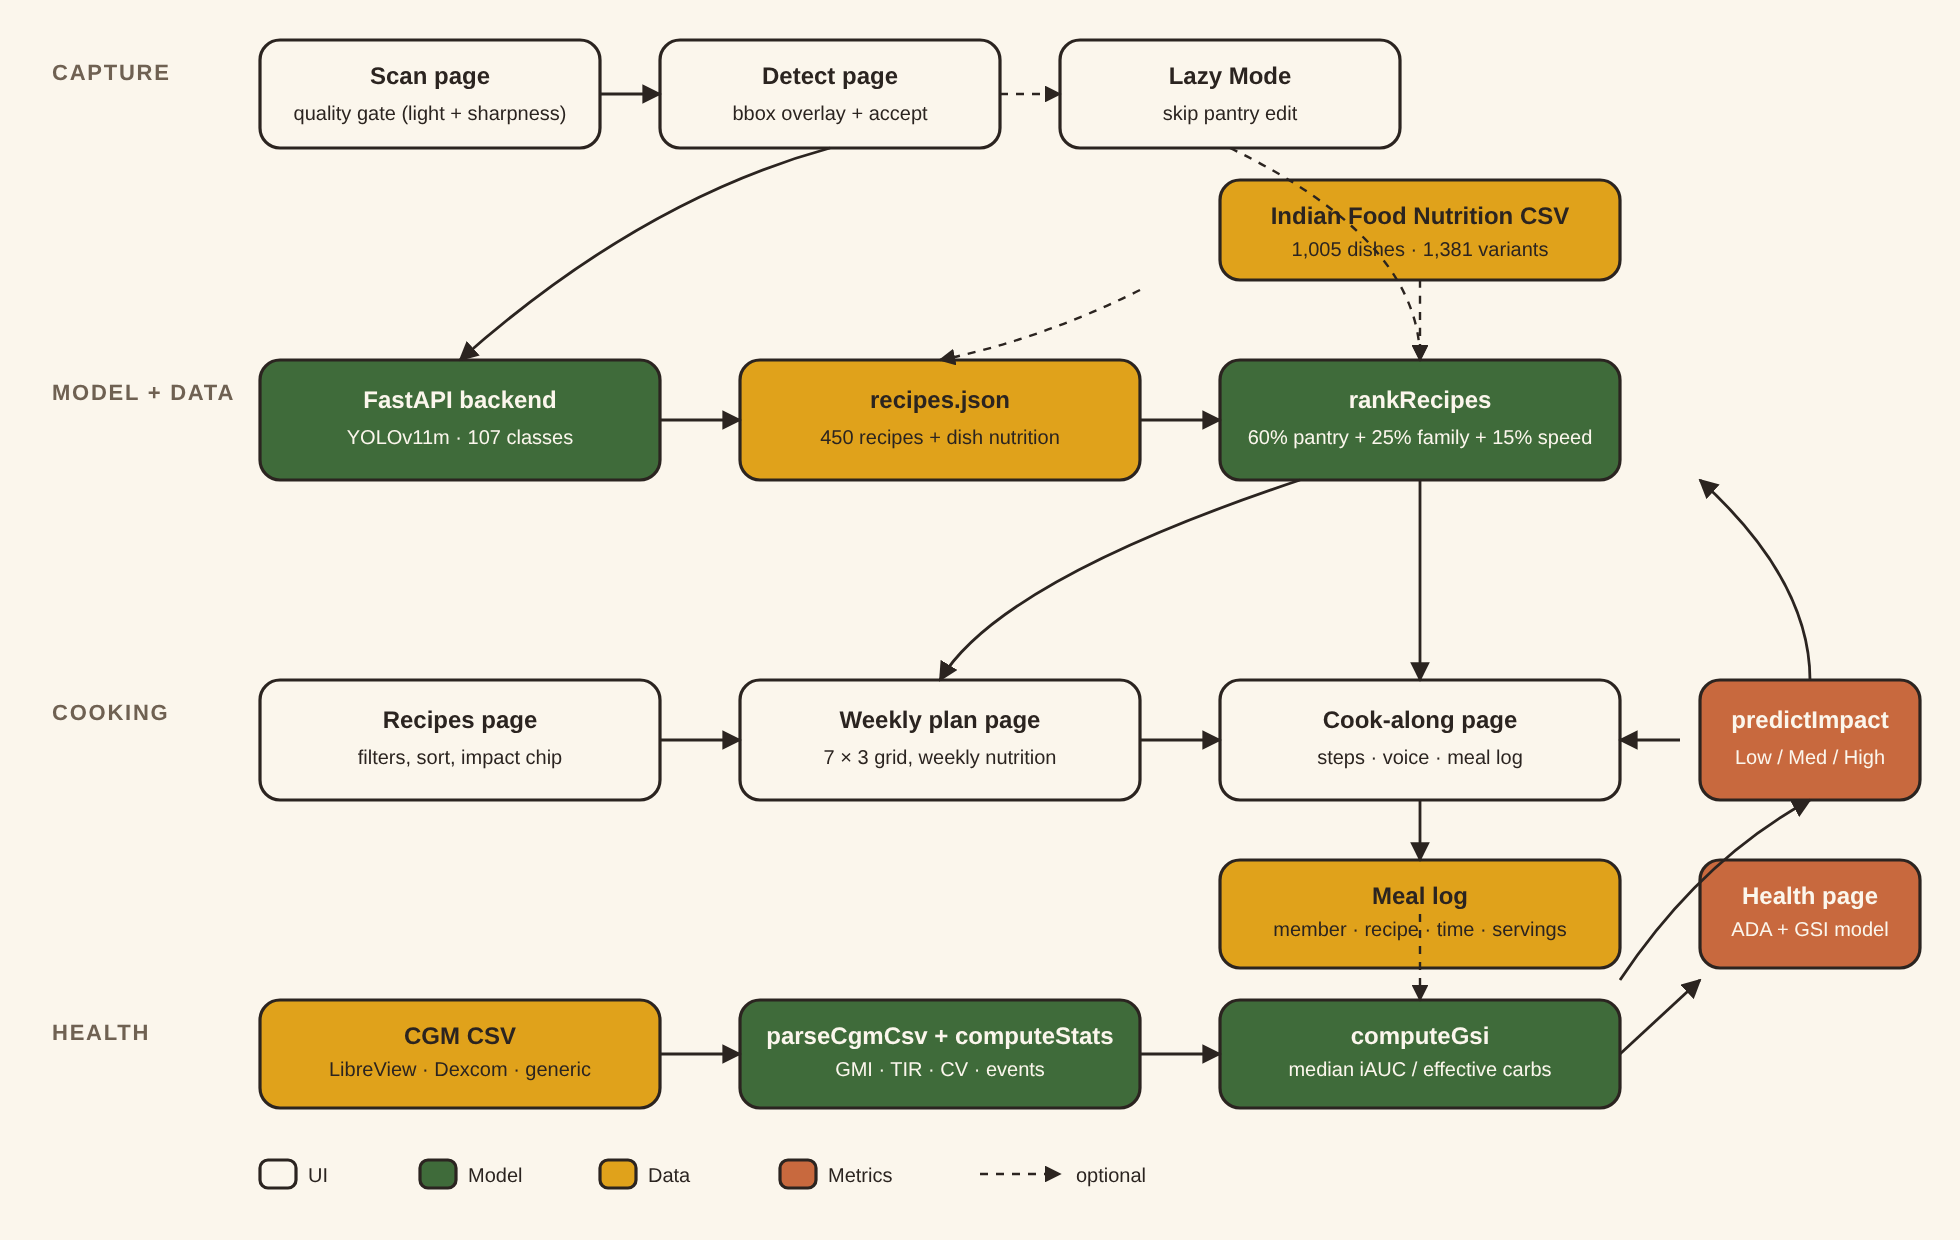
\includegraphics[width=0.96\textwidth]{figures/system_flow.png}
\caption{AHAAR end-to-end data flow. UI pages (cream), models
(green), data assets (amber), and output metrics (terracotta).
Solid arrows are mandatory data paths; dashed arrows are optional
(Lazy Mode skips the pantry edit; recipe nutrition is attached at
build time from the Indian Food Nutrition CSV; GSI feeds back into
the ranker as per-member impact chips). The single external
runtime dependency is the FastAPI inference server, which fits on
an RTX~3050 and can be substituted by the browser-ONNX pipeline
documented in \texttt{training/README.md} \S6.}
\label{fig:flow}
\end{figure*}

%====================================================================
\section{Evaluation Plan}
\label{sec:eval}

\begin{itemize}
  \item \textbf{Detection:} mAP@50, mAP@50:95, per-class precision
        and recall on AHAAR-Fridge val split, for all four ablation
        cells. Target: cell 3 (YOLOv11m + IF20 pretrain) exceeds the
        91.8\% mAP@50 reported by~\cite{indianfood10} on
        IndianFood10, demonstrating that the ingredient-level task
        is tractable and that two-stage transfer generalises.
  \item \textbf{Recipe retrieval:} Recall@1 and Recall@5 for a
        held-out 50-prompt query set (``I have X, Y, Z -- what
        can I cook?''), scored by the same \texttt{rankRecipes}
        used in production.
  \item \textbf{Nutrition enrichment:} coverage (fraction of recipes
        carrying a matched nutrition row -- currently 79\%) and
        hit-rate on a 15-dish gold-standard sanity test (currently
        14/15).
  \item \textbf{CGM metrics:} agreement of
        \texttt{src/lib/cgm.ts} with LibreView's own reported
        TIR/TBR/TAR on a real-world export, plus synthetic validation
        against \texttt{public/sample-cgm.csv} which is constructed
        with known ground-truth hyper and hypo events.
  \item \textbf{GSI learner:} leave-one-meal-out cross-validation
        of predicted iAUC against observed iAUC on 10 logged meals
        per diabetic member (small, illustrative).
  \item \textbf{System:} end-to-end latency on a Pixel-class phone
        and on a laptop, broken down per stage (scan $\rightarrow$
        detect $\rightarrow$ rank $\rightarrow$ render).
\end{itemize}

%====================================================================
\section{Discussion}
\label{sec:discussion}

AHAAR deliberately refuses two tempting shortcuts: (i) relying on an
off-the-shelf Indian food detector trained on plated meals, and
(ii) performing monocular volume estimation without a reference
object. The first is addressed by AHAAR-Fridge and the two-stage
transfer pipeline; the second is addressed by the standardised
reporting convention, which is honest about the limit.

The GSI-based recipe re-ranker is the project's most differentiated
contribution. It is the point at which AHAAR stops being yet another
recipe app and becomes a personalised health tool for the Indian
household. No current product combines Indian cuisine recipe
retrieval with CGM-driven glycemic personalisation.

\textbf{Threats to validity.} Our CGM evaluation dataset will be
small ($<$10 users); the GSI learner is illustrative, not clinical.
We state this limitation explicitly in the on-screen disclaimer, and
target a larger IRB-supervised study as future work. The rule-based
family-fit scoring is similarly honest: it draws on well-known
dietary guidance (DASH for BP, soluble fibre for cholesterol) but is
not a substitute for clinical advice.

%====================================================================
\section{Conclusion and Future Work}
\label{sec:conclusion}

We have presented AHAAR, a kitchen assistant for Indian households
that spans fridge scanning, ingredient detection, pantry management,
recipe recommendation, per-member portioning, weekly meal planning,
step-by-step cooking, and CGM-aware health personalisation. Every
page is backed by real code and real data; every design choice is
anchored in a peer-reviewed IEEE paper; the training pipeline
reproduces the paper's claimed metrics from a cold clone.

Future work includes: (i) scaling AHAAR-Fridge to 50 classes with
semi-supervised labelling; (ii) extending the GSI learner to a
regression-based model under IRB supervision on a type-2 diabetic
cohort; (iii) replacing the substring-based recipe matcher with a
learned im2recipe-style joint embedding over
Recipe1M+~\cite{marin2021recipe1m}; and (iv) adding an optional
reference-coin affordance for gram-accurate portion estimation.

%====================================================================
\section*{Acknowledgment}
The authors thank Ms.\ Sharlene Rebeiro for her guidance throughout
the project, and the open-source maintainers of Ultralytics YOLO,
FastAPI, React, TailwindCSS, i18next, Workbox, and PostgreSQL.

%====================================================================
\bibliographystyle{IEEEtran}
\bibliography{references}

\end{document}
